\chapter{Historie palubních počítačů}
Historicky, před vývojem digitální elektroniky, se provozní data vozidla meřila výhradně mechanicky a analogově. 
Příkladem je mechanický tachometr, poháněný ohebným hřídelem z převodovky. Rotační pohyb tohoto hřídele je přes soustavu ozubených kol přenášen na počítadlo ujeté vzdálenosti. 
Měření rychlosti bylo řešeno za využití vířivých proudů. Hřídel z převodovky otáčí magnetem vloženým do měděného nebo hliníkového prstence, ve kterém se indukují právě vířivé proudy. 
Vodivý prsten je spojen se střelkou tachometru ukazující rychlost vozidla. 

S nástupem prvních digitálních mikrokontrolérů v 70. letech začal i vývoj jednoúčelových palubních počítačů vozidel. 
Tyto systémy vozidlo neřídily, pouze poskytovaly data o provozu vozidla. Prvním takovým sériově vyráběným počítačem byl Cadillac Trip Computer ve vozidle Cadillac Seville.
Tento počítač umožňoval uživateli vypočítat průměrnou spotřebu paliva, rychlost vozidla, otáčky motoru, dojezd, zbývající čas příjezdu do finální destinace a další. \cite{gm1978trip}

\begin{figure}[htbp]
   \begin{center}
     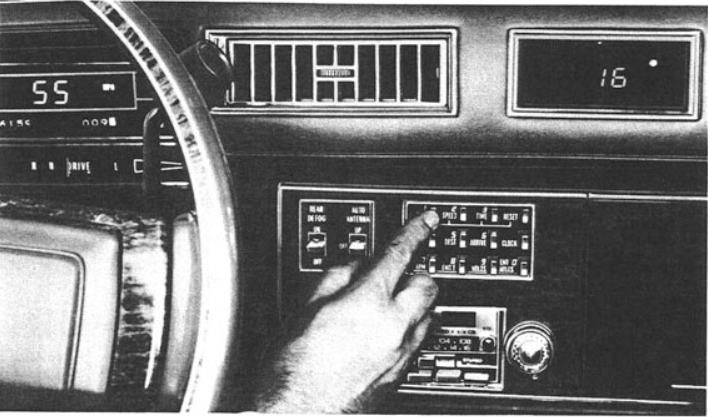
\includegraphics[scale=0.6]{obrazky/Cadillac_pocitac.png}
   \end{center}
   \caption[Fotografie počítače Cadillac Trip Computer]{Dobová fotografie počítače Cadillac Trip Computer (převzato z \cite{gm1978trip})}
 \end{figure}


\chapter{Současný stav problematiky}
V dnešní době se ve vozidlech může nacházet přes 70 řídících jednotek, které řídí veškeré systémy od motorů, přes stěrače, osvětlení, nebo odpružení vozidla až 
po veškeré asistenty a kamery\cite{navet2017automotive}. Zatímco moderní automobily disponují standardizovanými datovými sběrnicemi 
(např. CAN-Bus, FlexRay či Automotive Ethernet) a unifikovanými diagnostickými protokoly OBD-II, u vozidel starší výroby byla palubní elektronika silně 
proprietární a roztříštěná. V oblasti dodatečné montáže palubních počítačů se současný trh a amatérské komunity ubírají dvěma hlavními směry, 
které jsou popsány v následujících podkapitolách.  

\section{Univerzální přídavné palubní počítače}
Mezi komerčně dostupné univerzální přístroje patří především různé digitální budíky a head-up displeje určené pro připojení do standardizované diagnostické zásuvky OBD-II. 
Tyto přístroje jsou schopny v reálném čase číst provozní veličiny přímo z řídicí jednotky motoru. 
Jejich hlavní výhodou je plug-and-play instalace bez nutnosti jakýchkoliv zásahů do kabeláže vozidla.

Tato univerzální řešení však narážejí na zásadní technická omezení při použití na starších vozidlech, která nesplňují normu EOBD. 
Vozidla jako Škoda Felicia 1.3 MPI s řídicí jednotkou Siemens Simos 2P sice již disponují touto diagnostickou zásuvkou, avšak komunikace probíhá pomalým, 
proprietárním protokolem K-Line, který neposkytuje kontinuální datový proud provozních veličin ve formě standardních OBD-II veličin\cite{skoda_simos2p_1999}.

Z tohoto důvodu vznikají v rámci open-source komunity alternativní projekty, jako je například rozšířený systém MPGuino. 
Tyto přístroje fungují na principu externího měření – čtou šířku impulzů vstřikovacích ventilů a signál ze snímače rychlosti, na jejichž základě softwarově dopočítávají 
okamžitou a průměrnou spotřebu paliva.

\section{Dobový palubní počítač APRI TC-6}
Pro vozidla Škoda Felicia byl jako schválené originální příslušenství i jako volitelná tovární výbava dodáván palubní počítač s označením TC-6, 
vyvinutý českou společností APRI s.r.o..
Řídicí jednotky motorů vozidel Škoda Felicia (např. Siemens Simos 2P u motorizace 1.3 MPI či Bosch Mono-Motronic u 
starších verzí BMM\footnote{BMM - Řídící jednotka motorizace vozidla s jednobodovým vstřikováním paliva}) nedisponují datovou
sběrnicí CAN-Bus a jejich diagnostické rozhraní K-Line slouží primárně pro servisní diagnostiku přístrojem V.A.G 1552, nebo softwarem pro diagnostiku VCDS určeným pro vozy koncernu Volkswagen.
Z tohoto důvodu pracoval počítač TC-6 na principu přímého hardwarového snímání elektrických signálů z původní elektroinstalace vozidla\cite{skoda_simos2p_1999}.

Ovládání bylo řešeno pomocí dvojice tlačítek přímo na samotném počítači. Z hlediska zobrazovacích schopností využíval počítač TC-6 pasivní sedmisegmentový LCD displej s podsvícením,
který poskytoval informace o venkovní teplotě, okamžité a průměrné spotřebě paliva, stavu paliva, dojezdu vozidla, okamžité a průměrné rychlosti, době jízdy a palubním napětí.

Výroba kompletních sad byla již ukončena, dostupnost původních kabelových svazků a specifických senzorů na sekundárním trhu je minimální a třicet 
let staré moduly často vykazují degradaci tekutých krystalů displeje. 
Navrhovaný palubní počítač v této bakalářské práci proto vychází z osvědčené koncepce měřicích bodů systému TC-6, 
avšak implementuje ji na soudobé hardwarové platformě s moderním grafickým displejem.

\chapter{Získávání dat z vozidla bez datové sběrnice}

\section{Snímání rychlosti a ujeté vzdálenosti}
Ve vozidlech Škoda Felicia je informace o rychlosti přenášena z převodovky do přístrojového štítu čistě mechanicky pomocí ohebného hřídele. 
Tento hřídel uvnitř rychloměru roztáčí vícepólový válcový magnet. Kolem rotujícího magnetu je s minimální vzduchovou mezerou umístěn měděný vodivý bubínek, 
který je pevně spojen s ručičkou ukazatele. Změnou magnetického toku se v bubínku indukují vířivé proudy, 
které vytvářejí točivý moment a úměrně k rychlosti otáčení vychylují ukazatel proti síle vratné pružiny.

Pro účely elektronického zpracování rychlosti je využito konstrukční přípravy samotného rychloměru, 
který na své zadní straně disponuje technologickým otvorem. Do tohoto prostoru je situován Hallův snímač, 
který bezkontaktně detekuje střídání magnetických pólů rotujícího magnetu. Výstupem snímače je obdélníkový signál. 
Z frekvence tohoto signálu mikrokontrolér vypočítává okamžitou rychlost vozidla, zatímco čítáním absolutního počtu pulzů v čase se získává celková ujetá vzdálenost.

Vzhledem k uzavřené povaze a nedostupnosti původní technické dokumentace k dobovému počítači APRI TC-6 není přesná konstanta počtu pulzů na jeden ujetý kilometr z výroby známa. 
Návrh nového palubního počítače proto implementuje tuto hodnotu jako softwarově nastavitelnou kalibrační konstantu. 
Její přesná hodnota bude stanovena experimentálně během testovacích jízd a validována vůči referenčnímu modulu GPS.

\section{Měření otáček motoru}
Informace o otáčkách motoru je získávána přímo z nízkonapěťového signálu určeného pro přístrojový štít.
Z tohoto vedení lze číst spojitý obdélníkový signál, jehož frekvence je přímo úměrná rychlosti otáčení klikové hřídele. 
Pro výpočet otáček nelze využít frekvenci spínání vstřikovačů paliva, jelikož při brzdění motorem
řídicí jednotka vstřikování paliva zcela přeruší, což by vedlo k chybné interpretaci otáček motoru.

\section{Měření spotřeby paliva}
Měření spotřeby paliva je realizováno přímým monitoringem elektromagnetických vstřikovacích ventilů. 
Řídicí jednotka motoru reguluje množství dodaného paliva změnou šířky napěťového pulzu. 
Jelikož je mechanický průtok paliva ventilem při konstantním tlaku palivové soustavy fixní, lze celkovou spotřebu vypočítat přesným měřením doby, 
po kterou je vstřikovač elektricky sepnut.

Z historického hlediska řešil dobový počítač APRI TC-6 toto snímání neinvazivně pomocí externího indukčního snímače. 
Ten se mechanicky upínal na vodič vstřikovače a na principu proudového transformátoru detekoval napěťové špičky vznikající při prudkých změnách proudu. 
Ačkoliv toto řešení nevyžadovalo zásah do elektroinstalace, vykazovalo náchylnost k elektromagnetickému rušení z motorového prostoru a ztrátu citlivosti vlivem stárnutí.

Návrh nového palubního počítače proto volí metodu přímého měření elektrických úrovní prostřednictvím vřazeného mezikusu s konektory, 
což zachovává požadavek na neporušení originální kabeláže. Elektromagnetický vstřikovač s typickým odporem vinutí 15 až 20 $\Omega$ však představuje silnou indukční zátěž. 
Pro spolehlivou ochranu vstupů mikrokontroléru před vysokonapěťovými indukčními špičkami a pro čistý převod napěťových úrovní je ke snímání signálu vstřikovače využit optočlen, 
který mikrokontroléru předává bezpečné logické úrovně s časovou přesností. Průtok vstřikovače je v softwaru definován jako kalibrační konstanta, 
jež se doladí na základě reálných úbytků paliva v nádrži.

\section{Teplotní a další provozní snímače}
Zatímco otáčky motoru a rychlost vozidla představují dynamické pulzní signály, monitorování dalších provozních stavů vyžaduje zpracování spojitých analogových veličin. 
V kontextu starších vozidel se jedná především o následující parametry:

\begin{enumerate}
    \item \textbf{Napětí palubní sítě:} Měření stavu akumulátoru a dobíjecí soustavy spočívá ve snímání stejnosměrného napětí palubní sítě. 
    Jelikož maximální hodnoty tohoto napětí překračují logické úrovně moderních mikrokontrolérů, 
    je nezbytné signál před vstupem do A/D převodníku proporcionálně snížit. V praxi se k tomuto účelu využívá pasivní odporový dělič napětí, 
    jehož převodní charakteristika je lineární.
    \item \textbf{Snímání provozních teplot:} Pro měření teplot se v automobilovém průmyslu standardně využívají 
    termistory s negativním teplotním koeficientem. Odpor těchto polovodičových součástek nelineárně klesá s rostoucí teplotou. 
    Pro elektronické vyhodnocení je termistor typicky zapojen v sérii s referenčním rezistorem, čímž vzniká napěťový dělič. 
    Změna odporu senzoru se tak převádí na změnu úbytku napětí, kterou lze kvantifikovat pomocí A/D převodníku a softwarově linearizovat.
    \item \textbf{Měření hladiny paliva v nádrži:} Informace o zásobě paliva je v původní instalaci získávána z plovákového snímače, 
    který funguje na principu proměnného potenciometru. Tento senzor tvoří společně s ukazatelem na přístrojové desce uzavřený napěťový dělič. 
\end{enumerate}

\chapter{Specifika automobilové elektroniky}
Prostředí motorových vozidel představuje pro elektronická zařízení jeden z nejnáročnějších provozních scénářů. 
Při návrhu palubních přístrojů nelze aplikovat standardní postupy známé ze spotřební elektroniky, ale je nutné respektovat pravidla pro napájení, 
ochranu signálů a mechanickou odolnost.

\section{Napájení a napěťové špičky}
Palubní síť automobilu je zdrojem extrémního elektrického rušení. 
Největší hrozbou je tzv. Load dump efekt – masivní napěťová špička, která vznikne při odpojení vybitého akumulátoru v momentě, kdy alternátor dodává vysoký proud. 
Tyto špičky mohou dosahovat desítek voltů a trvat stovky milisekund. Vstupní napájecí kaskáda proto musí být teoreticky vybavena prvkem pro potlačení přechodových jevů, 
typicky TVS diodou \footnote{TVS - Transient Voltage Suppressor}.

Z hlediska energetické efektivity je nevhodné snižovat palubní napětí na logické úrovně pouze lineárními stabilizátory, 
které by přebytečný výkon měnily ve vysoké množství tepla. Ideálním teoretickým modelem je dvoustupňová kaskáda: primární spínací měnič zajišťuje vysokou 
účinnost přeměny na 5 V, zatímco sekundární lineární stabilizátor s nízkým úbytkem napětí následně vyhlazuje zbytkové zvlnění a poskytuje precizní a čisté napětí 3,3 V 
pro citlivé měřicí obvody.

\section{Ochrana signálových vstupů a filtrace rušení}
Kromě napájení je nutné chránit i samotné datové a měřicí vstupy, na které se indukují rušivá napětí ze zapalovací soustavy a spínání indukčních zátěží. 
Teorie návrhu automobilové elektroniky definuje tři základní pilíře ochrany:

\begin{enumerate}
    \item \textbf{Galvanické oddělení:} Kde je to technologicky možné, využívají se pro digitální signály optočleny, 
    které tvoří fyzickou bariéru proti vysokému napětí a slouží jako bezztrátové převodníky napěťových úrovní.
    \item \textbf{Omezení napětí:} Analogové vstupy k A/D převodníkům musí být chráněny, typicky pomocí Zenerových diod. 
    Ty zajistí, že napětí na pinu nikdy nepřekročí maximální referenční hodnotu, čímž se zabrání destrukci vstupních hradel mikrokontroléru.
    \item \textbf{Vysokofrekvenční filtrace:} Plošný spoj musí být osazen blokovacími a filtračními kondenzátory umístěnými co nejblíže 
    napájecím a signálovým pinům integrovaných obvodů.
\end{enumerate}

\section{Klimatické a mechanické vlivy}
Automobil prochází extrémními teplotními cykly. Ačkoliv je řídicí jednotka palubního počítače umístěna v interiéru vozidla, čímž je chráněna před nejvyššími teplotami 
motorového prostoru, interiér uzavřeného vozu v letních měsících běžně dosahuje velmi vysokých teplot, zatímco v zimě klesá pod bod mrazu. 
Všechny polovodičové komponenty proto musí teoreticky splňovat minimálně rozšířený teplotní rozsah.

Z hlediska mechanického namáhání podléhá zařízení neustálým vibracím od motoru a rázům od vozovky. 
Použití standardních násuvných propojek by mohlo být riskantní. 
Pro zajištění dlouhodobé spolehlivosti systému je vyžadováno použití konektorů s mechanickou aretací, které zabraňují 
samovolnému rozpojení spojů a zajišťují stálý přítlak kontaktů.

\chapter{Legislativní a bezpečnostní aspekty zástavby}
%Při návrhu jakéhokoliv elektronického zařízení určeného pro provoz v silničním vozidle je nezbytné zohlednit nejen funkční požadavky, ale také platný legislativní rámec, 
%podmínky technické způsobilosti vozidla a elektrickou bezpečnost palubní sítě. Neodborný, nebo trvalý zásah do elektroinstalace může vést ke ztrátě technické způsobilosti vozidla
%při pravidelné kontrole na stanici technické kontroly, případně poškození řídících systémů.

%\section{Homologace a koncepce funkčního vzorku}
%V České republice jsou podmínky provozu vozidel na pozemních komunikacích upraveny zákonem č. 56/2001 Sb. \cite{zakon56_2001} a prováděcí vyhláškou č. 153/2023 Sb., o schvalování technické způsobilosti
%vozidel\cite{vyhlaska153_2023}. Z hlediska automobilové elektroniky je klíčovým dokumentem předpis EHK OSN č. 10\cite{ehk10_emc}, který stanovuje požadavky na elektromagnetickou kompatibilitu.
%Tento předpis rozlišuje přídavné elektronické podskupiny, které při pevném spojení s vozidlem a prodeji na komerčním trhu vyžadují typové schválení.

%Vzhledem k tomu, že předmětem této práce je vývoj individuálního funkčního vzorku pro experimentální a diagnostické účely, není certifikace v akreditované zkušebně ekonomicky
%realizovatelná. Aby navržený palubní počítač plně vyhovoval legislativním požadavkům a nevyžadoval zápis změny do technického průkazu vozidla, je celé zařízení koncipováno
%jako modulární a plně odnímatelné příslušenství s čistě pasivním charakterem měření.

%\section{Požadavky z hlediska metodiky kontrol STK}
%Metodika a rozsah kontrolních úkonů prováděných na stanicích technické kontroly jsou definovány vyhláškou č. 211/2018 Sb., o technických prohlídkách vozidel\cite{vyhlaska211_2018}. Na základě
%analýzy prílohy č. 1 této vyhlášky byly při návrhu palubního počítače zohledněny tři kritické oblasti:

%\begin{enumerate}
%  \item \textbf{Výhled řidiče a pasivní bezpečnost interiéru:} Zobrazovací jednotka nesmí zasahovat do stírané plochy čelního skla ani omezovat přímý výhled řidiče z vozidla.
%      Konstrukce krytu zařízení je navržena bez ostrých hran a je umístěna mimo zóny dopadu hlavy a dráhy aktivace zádržných systémů.
%  \item \textbf{Bezpečnost elektrické instalace:} Dodatečně instalované vodiče nesmí vykazovat poškození izolace, nesmí být vedeny v blízkosti pohyblivých či tepelně namáhaných
%      částí motoru a musí být řádně vyvázány k původním kabelovým svazkům v ochranné bužírce. Napájecí větev odebíraná z 12V akumulátoru je bezprostředně u zdroje jištěna
%      vlastní tavnou pojistkou, která v případě zkratu na kostru vozidla zamezí tepelnému poškození vodiče či vzniku požáru.
%  \item \textbf{Nulový vliv na řízení motoru a emise:} Při měření emisí a vyčítání paměti závad řídící jednotky motoru nesmí přídavné zařízení způsobovat chybová hlášení
%      ani ovlivňovat přípravu palivové směsi. Navržený systém proto pracuje výhradně v režimu pasivního čtení a do řízení akčních členů nijak nezasahuje.
%\end{enumerate}

%\section{Elektrické oddělení měřených obvodů a odolnost v palubní síti}
%Palubní síť automobilu představuje z hlediska elektrického rušení a přechodových jevů vysoce náročné prostředí, které popisuje norma ČSN ISO 7637-2\cite{iso7637_2}. Při spínání indukčníchzátěží vznikají v síti napěťové špičky, které mohou dosahovat desítek voltů. Vstupní napájecí kaskáda navrženého zařízení je proto vybavena ochranou proti přepólování,
%transilem pro potlačení napěťových špiček a spínaným snižujícím měničem.

%Zvláštní pozornost byla věnována neinvazivnímu snímání signálů z originálních senzorů a akčních členů vozu:

%\begin{enumerate}
%  \item \textbf{Snímání doby sepnutí vstřikovačů:} Elektromagnetický vstřikovač paliva představuje indukční zátěž s odporem vinutí typicky v rozmezí 15 až 20~$\Omega$,
%      při jejímž rozepnutí vznikají napěťové špičky přesahující 60 V\cite{skoda_simos2p_1999}. Měřící vstup je proto oddělen optočlenem (více viz kapitola Měření spotřeby paliva).

%  \item \textbf{Měření hladiny paliva v nádrži:} Snímač hladiny paliva pracuje na principu odporového potenciometru, ovládaného plovákem, který je zapojen do napěťového děliče
%      originální přístrojové desky. Aby paralelní spojení palubního počítače nezměnilo impedanci obvodu a tím nezkreslilo údaj původního palivoměru, je signál snímán přes
%      oddělovací obvod s velmi vysokou impedancí (více viz kapitola Měření hladiny paliva v nádrži).
%\end{enumerate}